\documentclass[11pt]{article}

\usepackage[left=3cm,right=3cm,top=3cm,bottom=3cm]{geometry}

% For Times New Roman font
\usepackage{mathptmx}

% Packages for formatting
\usepackage{titlesec}
\usepackage{titling}
\usepackage{abstract}

\usepackage{algorithm}
\usepackage{algpseudocode}
\usepackage{float}
\usepackage{anyfontsize}
\usepackage{etoolbox}
\usepackage{graphicx}
\usepackage{tcolorbox}
\usepackage{enumitem}

% Customize section and subsection font sizes
\titleformat{\section}[block]{\normalfont\fontsize{13pt}{15pt}\bfseries}{\thesection}{1em}{}
\titleformat{\subsection}[block]{\normalfont\fontsize{12pt}{14pt}\bfseries}{\thesubsection}{1em}{}

% Change the title font size
\pretitle{\vspace{-6em}\begin{center}\fontsize{14pt}{16pt}\bfseries}
\posttitle{\par\end{center}\vskip 0.5em}

\preauthor{\vspace{0em}\begin{center}\small}
\postauthor{\vspace{-4em}\end{center}}

\renewcommand{\abstractname}{}
\renewcommand{\abstractnamefont}{\normalfont\small\bfseries}
\renewcommand{\abstracttextfont}{\normalfont\small}


% Remove line numbers
\makeatletter
\patchcmd{\algorithmic}{\itemsep\z@}{\itemsep\z@\lineskip\z@}{}{}
\makeatother


\begin{document}

\title{Indexus: A Peer-to-Peer Data Indexing System}
\author{Remi Henriot  \\
        www.indexus.io \\
        Draft version: 0.0.1}
\date{}

\maketitle

\begin{abstract}
\noindent \textbf{Abstract. }A peer-to-peer protocol engineered to facilitate nearest neighbors and range queries across multi-dimensional datasets. Both node addresses and datasets are mapped onto a unified binary space partitioning (BSP) tree, creating a streamlined and convergent system. The choice of a BSP tree over an R-tree for the data splitting strategy simplifies the protocol by reducing complex node interactions during insertion and deletion operations. The system achieves eventual consistency, high I/O throughput, and robust resilience through the integration of CRDT mechanisms, complemented by strategic caching and replication.
\vspace{1em}\end{abstract}

\section*{Introduction}
In the contemporary digital ecosystem, the concentration of data control by a limited number of centralized entities poses significant risks, including privacy violations and the potential for abuse of power. These entities create systemic vulnerabilities due to their centralized nature, which can lead to significant data breaches and a lack of competitive diversity in the market.

Advancements in decentralized technologies have begun to address these issues by enabling secure, transparent transactions and autonomous data management without centralized oversight. These innovations have facilitated more democratic governance structures and provided mechanisms for asset digitization, contributing to a more equitable digital landscape.

However, a critical challenge persists: the user experience in decentralized systems often lacks the ease and efficiency of data retrieval found in centralized platforms. Centralized systems benefit from advanced indexing systems that facilitate straightforward navigation and information retrieval, a feature decentralized architectures have struggled to match.

To bridge this gap, there is a need for a decentralized protocol that integrates a global indexing layer. Such a protocol would enhance the functionality of decentralized networks, making them more accessible and user-friendly. This improvement is crucial for increasing the adoption of decentralized solutions, thus supporting a shift towards a more distributed and resilient digital infrastructure.

\section*{Objective and constraints}
We aim to develop a data storage and retrieval system that organizes data in way incremental nearby search is possible to mimic existing data feeds. 
If we consider a news feed scroll it begins at the present moment—the spatial origin—and progresses backwards in time. As users scroll, they encounter older news items that are incrementally distanced from the origin.

Any feed, whether it tracks events or operates as part of an online marketplace, can be conceptualized as a single or multi-dimensional incremental search. The underlying data reservoir for these feeds can be vast, necessitating a system that can handle intensive read and write operations robustly. To ensure equitable data access and prevent centralized control, the data should not be localized on a single machine. Instead, it must be distributed across a network of nodes, supporting a decentralized architecture that avoids unfair ownership and enhances system resilience.

For this system, the immediate consistency of the feed is not critical, provided that the data eventually converge to a stable state. This approach allows for eventual consistency across the network, enabling the system to prioritize performance and scalability while ensuring that nodes will ultimately synchronize to reflect coherent information.

\section*{Structure}

The client and node interactions rely on the same data structure: a binary tree representing the encoding space where node addresses, collection ids, sets and item locations are materialized by the leaves of the tree. The data structure has been chosen carrefully to support collection scalability, search queries and network routing.

\vspace{1em}

\begin{figure}[H]
    \centering
    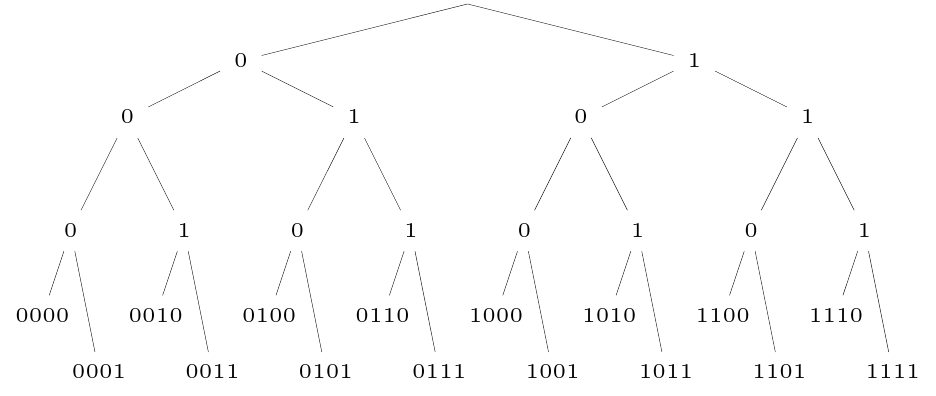
\includegraphics[width=10cm]{tree.png}
    \label{fig:tree}
    \caption{Binary tree}
\end{figure}

\vspace{1em}

Let’s consider a BASE4 system (using symbols A, B, C, and D) for our examples. The size of the base determines the amount of data stored within each set. Typically, we use a base 64 system for greater efficiency.

\vspace{1em}

\begin{figure}[H]
    \centering
    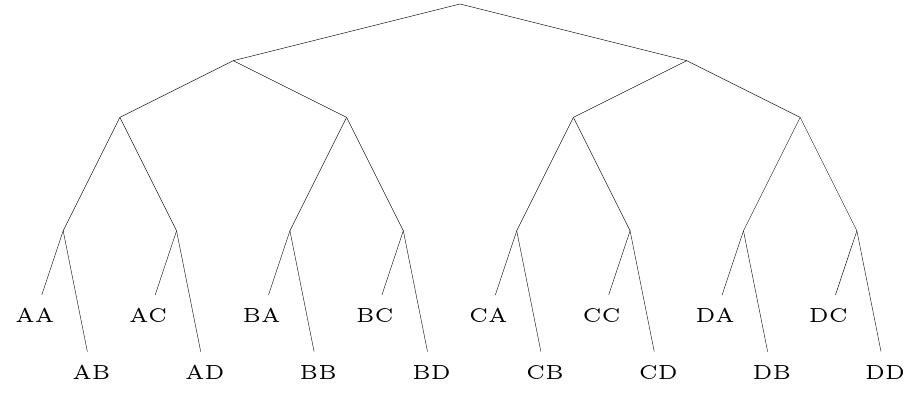
\includegraphics[width=10cm]{encoded.png}
    \label{fig:encoded}
    \caption{Encoded tree (BASE4)}
\end{figure}

\vspace{1em}

\section*{Network}

A node is a machine participating in the protocol. Its address is encoded from the cryptographic public key it has generated to prove its authencity over the network. Nodes are affected collection root sets or delegated subsets based on their addresses. They maintain a routing table to interact with other peers and enable clients to do so.

\vspace{1em}

\begin{figure}[H]
    \centering
    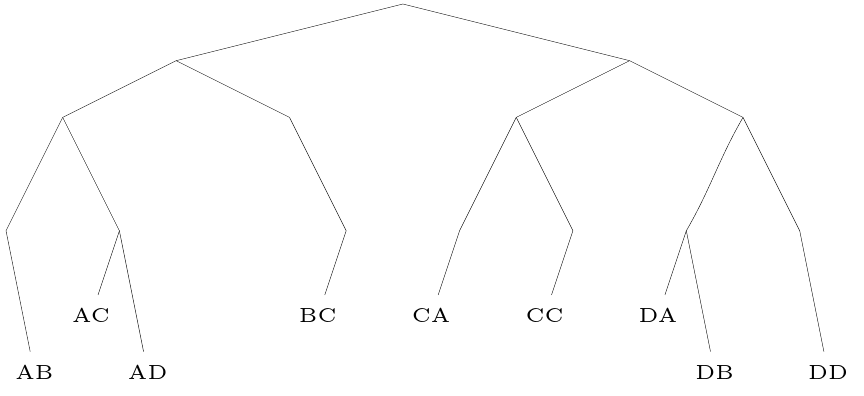
\includegraphics[width=10cm]{network.png}
    \label{fig:network}
    \caption{Network of nodes}
\end{figure}

The protocol relies on a routing table organized into \( N \) buckets, each designed to hold up to \( k \) node addresses. The buckets categorize nodes based on distance metrics (XOR metric), optimizing the network for efficient data retrieval and robust connectivity. The parameters \( N \) and \( k \) correspond to the number of buckets and the maximum number of nodes per bucket, respectively.

\vspace{1em}

\begin{figure}[H]
    \centering
    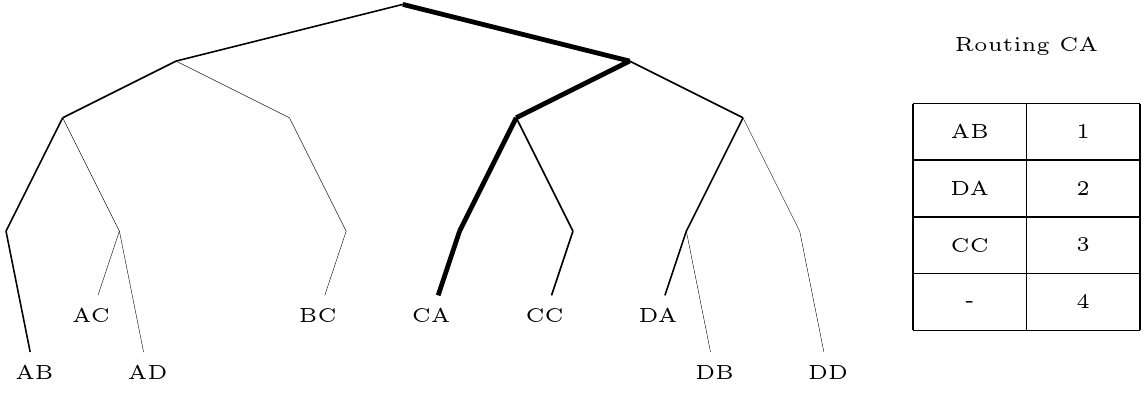
\includegraphics[width=13cm]{routing.png}
    \label{fig:routing}
    \caption{Routing table (N=4, k=1)}
\end{figure}

\subsection*{Example}
Let's represent a collection and its data with the following parameters - dimensions: 2, base: 4, set size: 10, properties: [count], offset: none

\vspace{1em}

\begin{figure}[H]
    \centering
    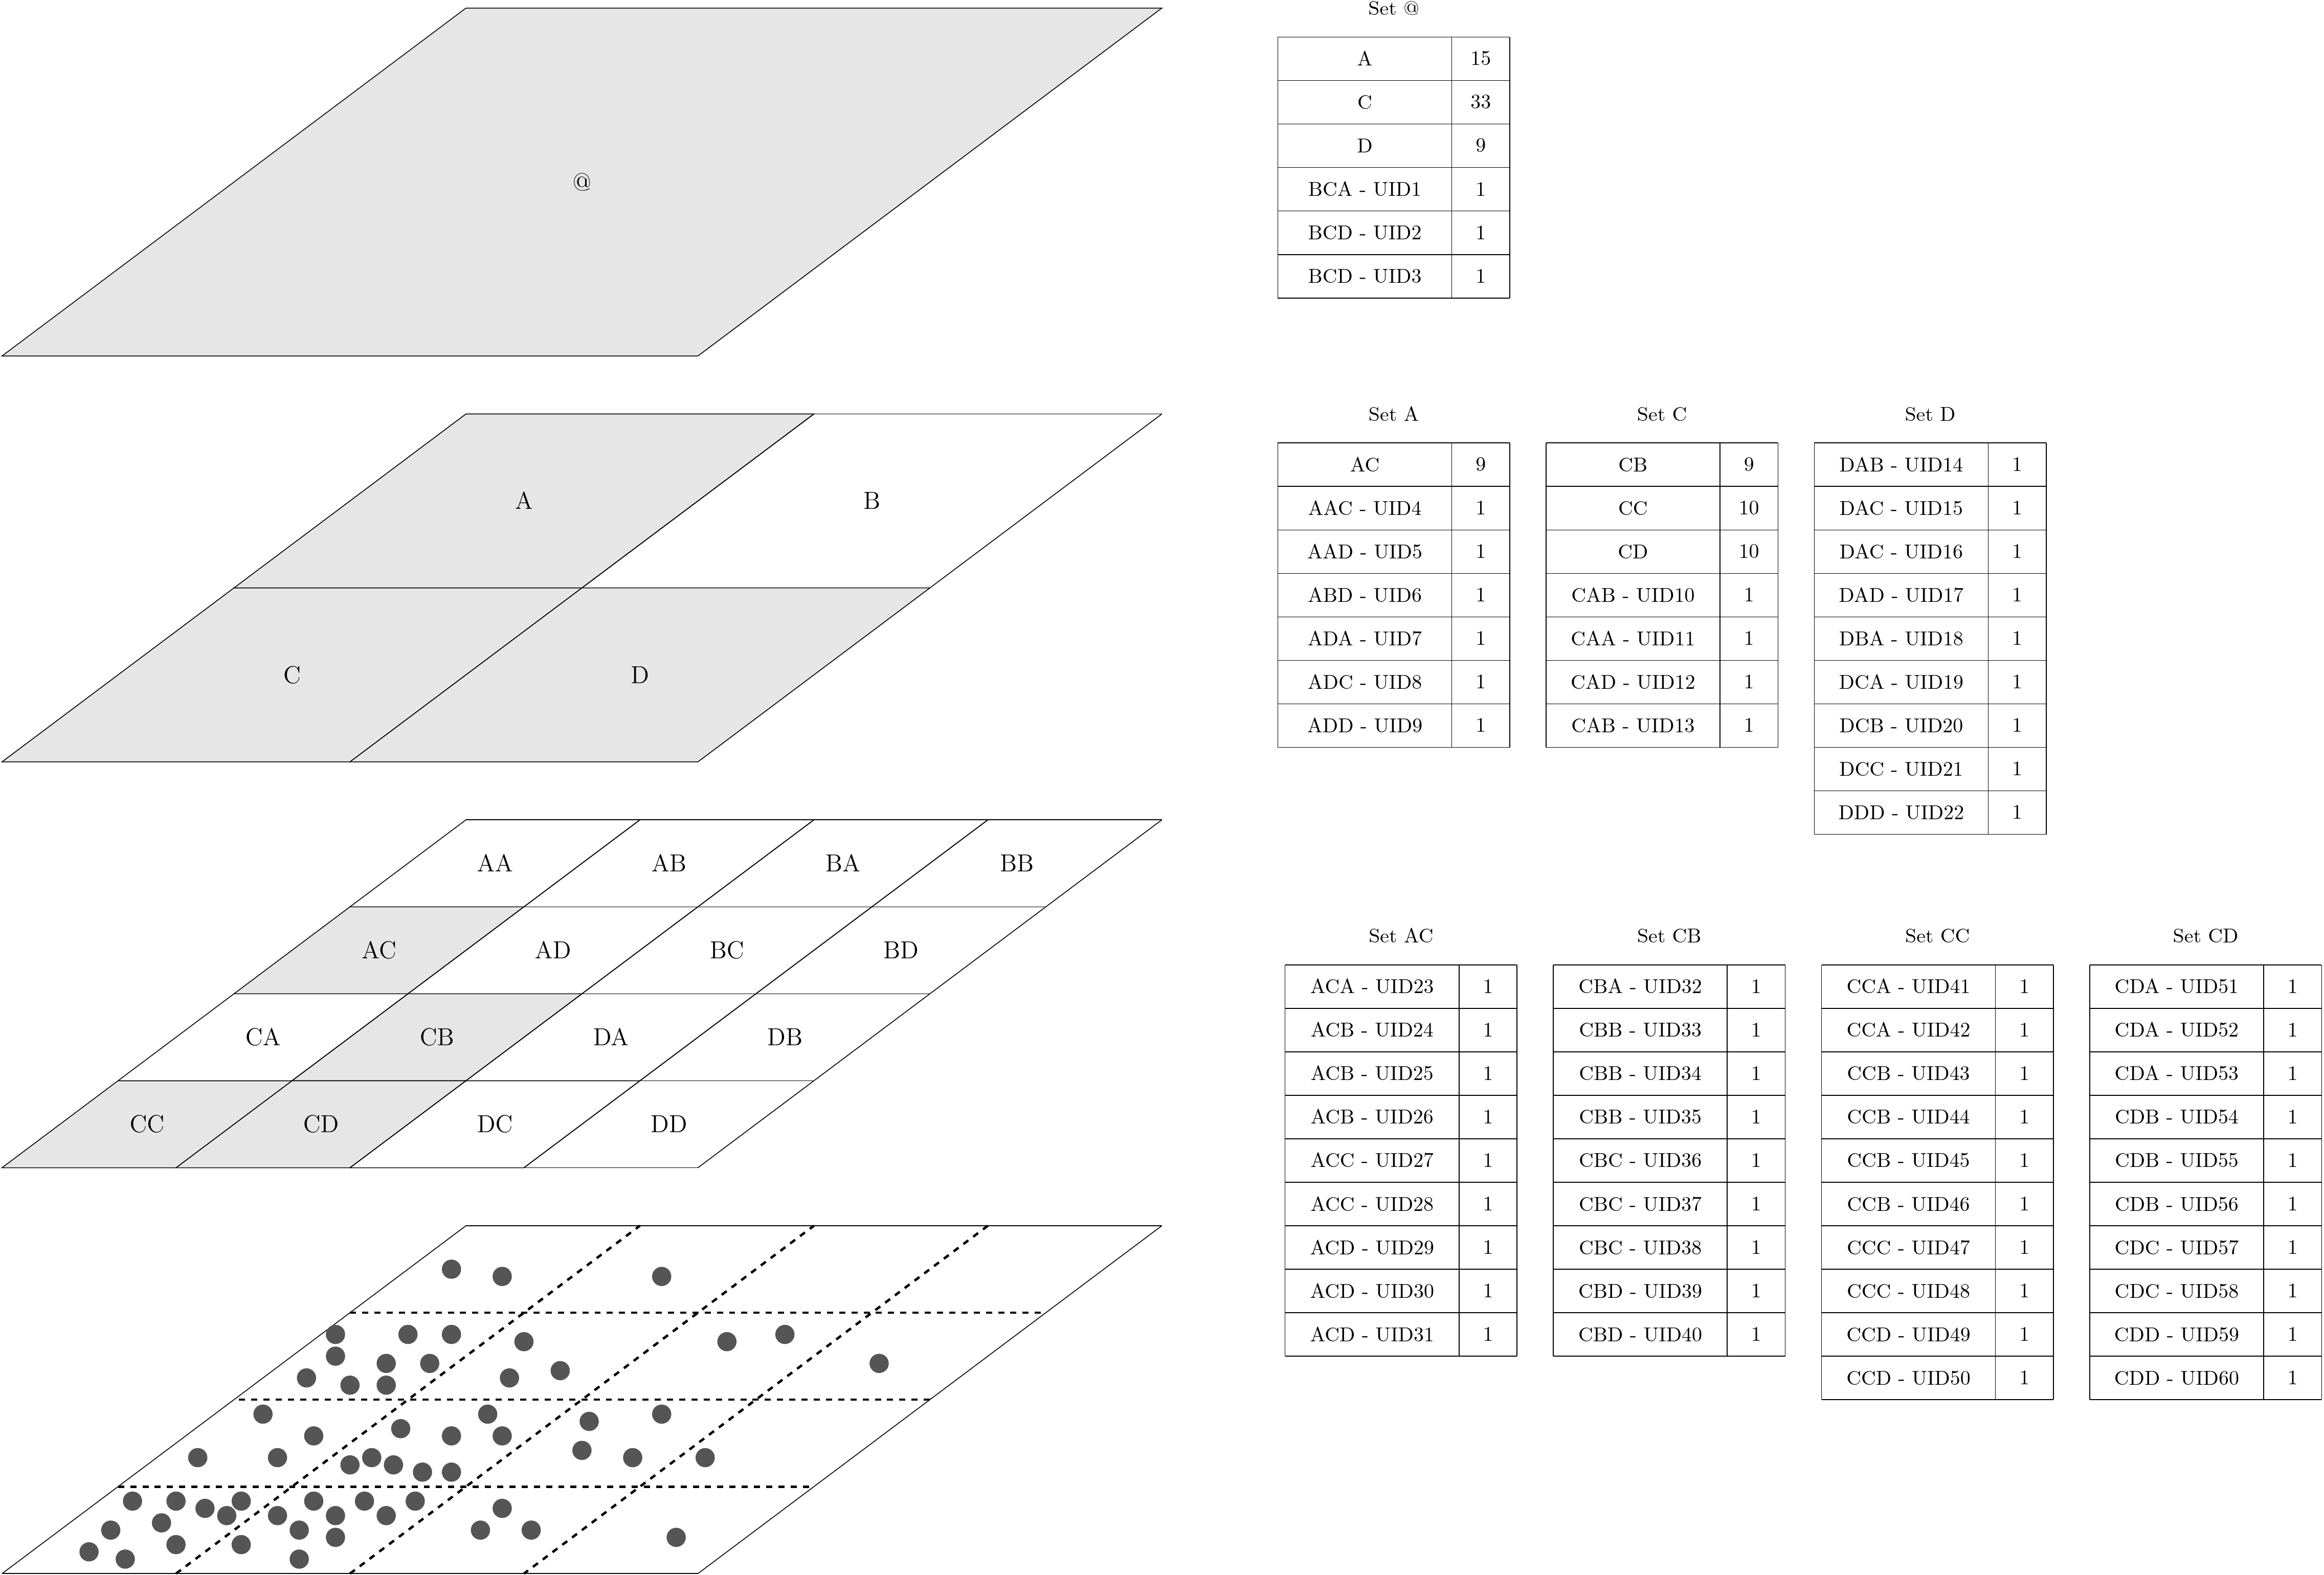
\includegraphics[width=15cm]{collection.png}
    \label{fig:collection}
    \caption{Collection, set and items}
\end{figure}

\vspace{2em}

\section*{Delegation mechanism}

We want to describe the data delegation for a collection over a static network of nodes. We chose a collection with the following paramters - dimensions: 2, delegation limit: D, base: 4, offset/ID: BB

\vspace{1em}

The network of nodes and collection data are represented over a binary tree, thick lines to the nodes supporting the collection and dashed lines to the delegated sets locations. We display multiple layers and tiles to represent the delegated sets, they are represented without the offset encoding for simplicity. Darker tiles are the delegated ones, meaning the total number of child items is greater than or equal to D.

\small
\subsection*{State at t1}
Tile @ → Leaf BB → Node BC\\

\begin{figure}[H]
    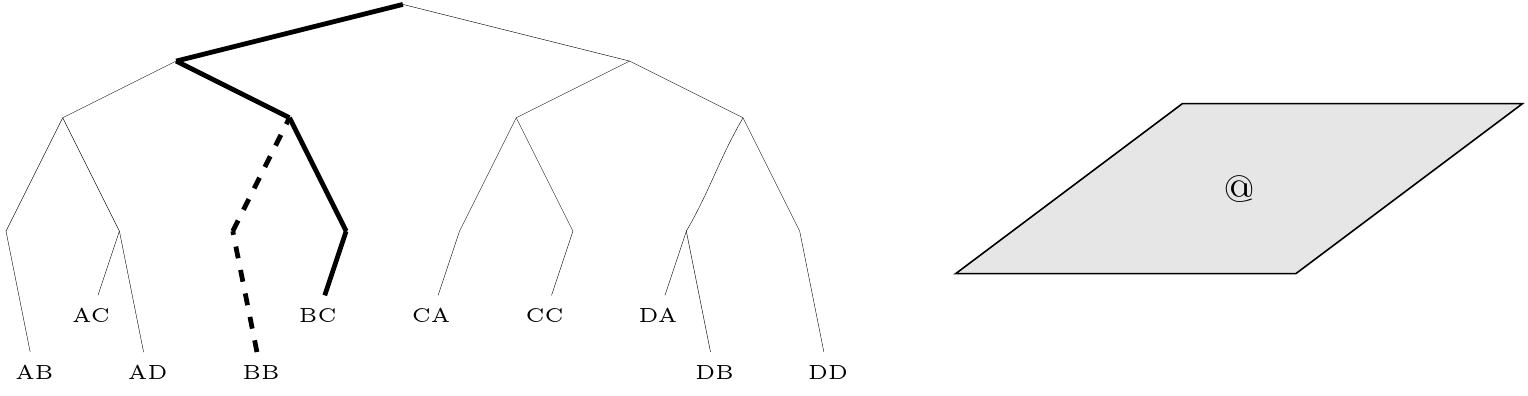
\includegraphics[width=13cm]{delegation-1.png}
    \label{fig:delegation_1}
    \caption{Delegation - representation at t1}
\end{figure}

\vspace{2em}

\subsection*{State at t2}
Tile @ → Leaf BB → Node BC\\
Tile A → Leaf AB → Node AB\\
Tile C → Leaf CB → Node CA\\

\begin{figure}[H]
    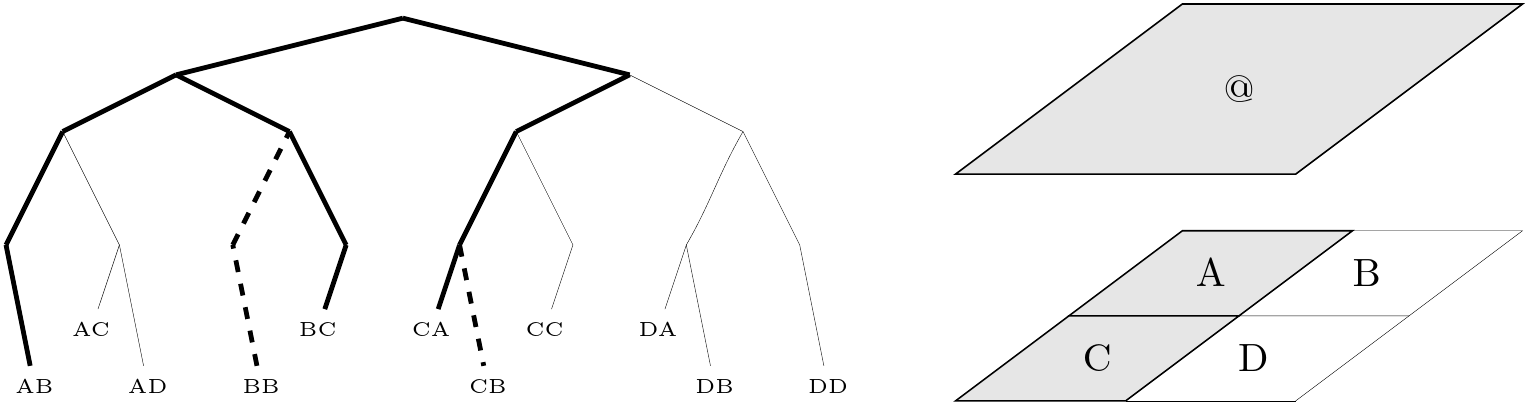
\includegraphics[width=13cm]{delegation-2.png}
    \label{fig:delegation_2}
    \caption{Delegation - representation at t2}
\end{figure}

\vspace{2em}

\subsection*{State at t3}
Tile @  → Leaf BB → Node BC\\
Tile A  → Leaf AB → Node AB\\
Tile C  → Leaf CB → Node CA\\
Tile D  → Leaf DB → Node DB\\
Tile AC → Leaf AC → Node AC\\
Tile CB → Leaf CB → Node CA\\
Tile CC → Leaf CC → Node CC\\
Tile CD → Leaf CD → Node CC\\

\begin{figure}[H]
    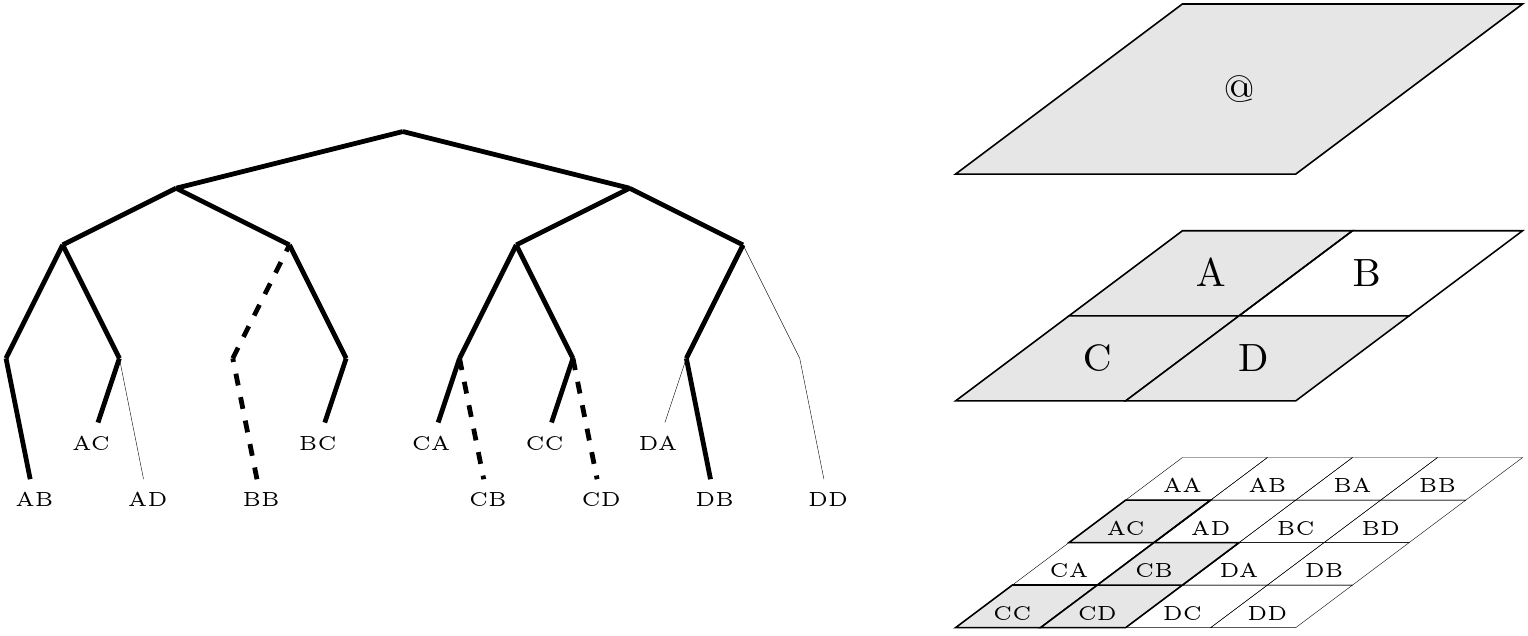
\includegraphics[width=13cm]{delegation-3.png}
    \label{fig:delegation_3}
    \caption{Delegation - representation at t3}
\end{figure}

\vspace{2em}

\normalfont

\section*{Following ideas are in draft mode and should be considered as implementation decisions for now}

\section*{Conflict resolution (already implemented)}
The network of nodes can be split and therefore the delegation mechanism need a way to resolve conflict or resolved inconsistencies when the network itself has been repaired. 

\section*{Synchronization (already implemented)}
To ensure the data converge to a consistent state, counts and properties need to be synchronized accross nodes when delegation happens. We propose to perform this operation concurrently with the routing protocol operations. Different strategies could be adopted based on the responsiveness constraints required. 

\section*{Replication (not yet implemented)}
A replica is the complete data stored within a single node so in case of failure we can recover all of it.

\section*{Caching (already implemented)}
An requests corresponding to a unkown set will replay the contact details of a closer node and might also decide after repeated requests to cache the original data and query also its closer contact. It allows the network to balance the read throughput to multiple nodes instead of one.

\section*{Topologies}
One network of nodes should be called a topology: space of addresses should have the same synchronization parameters, numbers of replicas, caching strategies, base used for the binary tree, length of the id for all collections, (potentially retribution mechanism and other things).


\end{document}